\section{SPI}
E' un' altra periferica di comunicazione pensata per brevi distanze ed alte velocità.

\begin{figure}[H]
    \centering
    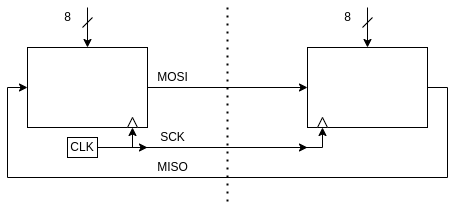
\includegraphics[width=300px]{images/23_SPI/SPI.png}
\end{figure}

Si utilizzano 3 fili per comunicare:
\begin{itemize}
    \item SCK: serial clock
    \item MOSI: master output slave input
    \item MISO: master input slave output
\end{itemize}
Ci può essere anche un altro filo detto \verb{SS{ che sta per slave-select.

I singoli dispositivi non sono altro che degli shift register, ad ogni impulso di clock dal primo dispositivo esce un bit ed entra nel secondo dispositivo e dal secondo dispositivo esce un bit che entra nel primo dispositivo.
Dopo 8 impulsi di clock i due dispositivi si sono scambiati un byte di dati.

Come si può notare questo protocollo di comunicazione è intrinsecamente bidirezionale, ogni trasmissione è anche una ricezione.

La velocità in genere è di qualche MHz e si comunica per massimo qualche centimetro.

Il clock è prodotto da un solo dispositivo che lo produce per se stesso ed anche per l' altro dispositivo, chi emette il clock è il master, chi lo riceve è uno slave.

Si noti che se io devo solo leggere ma non scrivere mi basta inviare gibberish (dummy byte), lo slave saprà cosa farsene eventualmente.

Anche in questo protocollo la trasmissione avviene per trama in quanto si inviano tutti gli 8 bit uno appresso all' altro.
Per alcune versioni di SPI i registri e quindi le trame sono a 16 bit.

Per trasmettere bisogna scrivere un byte nello shift register, a tal punto la logica si attiva ed abilita il clock per 8 impulsi, dopo gli impulsi la comunicazione è avvenuta e conclusa.

E' possibile che quando i dispositivi sono a pari livello (come due microcontrollori) il master non sia sempre lo stesso dispositivo ma cambi.
Per fare ciò si utilizza il filo SS, occorre modificare il codice di entrambi i dispositivi in modo da scegliere quale debba essere il master se sulla linea è posto 1 e chi debba esserlo se la linea è a 0.
Questa modalità è detta \emph{multi-master}.

Si noti che una volta ricevuto qualcosa il dato va letto subito in quanto al prossimo bit il contenuto è perso, per risolvere questo problema e dare più tempo in ricezione c'è un double buffer quindi una volta ricevuto un dato viene posto in un secondo buffer, finché non finisce la ricezione del secondo dato questo buffer continua ad essere coerente, abbiamo il tempo per leggerlo pari ad una intera trama anziché il singolo bit.

La frequenza di clock è libera in quanto a generarla è il master, non deve essere standard.

\subsection{Registri}
\subsubsection{SPCR}
\begin{figure}[H]
    \centering
    
\includegraphics[width=320px]{images/23_SPI/SPCR.png}
\end{figure}
\begin{itemize}
    \item SPIE: abilita l' interruzione quando:
    \begin{itemize}
        \item se siamo master quando completiamo la trasmissione (e ricezione)
        \item se siamo master quando l' arbitro ci costringe a diventare slave durante una trasmissione, che viene abortita
        \item se siamo slave quando completiamo una ricezione (e trasmissione)
    \end{itemize}
    \item SPE: abilita la periferica SPI
    \item DORD: data order, ci permette di scegliere la endianness della trasmissione
    \item MSTR: indica se vogliamo essere master o slave.
    Per decidere se dobbiamo seguire le decisioni dell' arbitro o continuare a seguire la configurazione che diamo noi si deve impostare correttamente il pin SS.
    Se lo impostiamo come ingresso allora seguiamo l' hardware, se lo impostiamo come uscita allora imponiamo la nostra decisione
    \item CPOL: clock polarity, si usa per indicare se il clock in idle deve essere a 0 (quindi l' impulso è un picco positivo) o a 1 (quindi l' impulso è un picco negativo)
    \item CPHA: clock phase, si usa per indicare se devo memorizzare sul primo fronte o sul secondo
    \item SPR2/1/0: servono per scegliere il prescaler da usare per generare il clock della trasmissione a partire dal clock del uC 
\end{itemize}

\subsubsection{SPSR}
\begin{figure}[H]
    \centering
    
\includegraphics[width=320px]{images/23_SPI/SPSR.png}
\end{figure}
\begin{itemize}
    \item SPIF: è il flag dell' interruzione pendente
    \item WCOL: ci dice se c'è stata una collisione cioè se abbiamo scritto sullo shift register mentre era in corso una trasmissione
\end{itemize}

\subsubsection{SPDR}
Registro all' interno del quale si inserisce il byte da inviare, alla scrittura viene anche avviata la trasmissione.


